\section{Mockups}



\subsection{\labeltext[Ecrã - Home]{Ecrã - Home}{mo:270}}

Esta será a primeira pagina do nosso frontend. A home página com as funcionalidades do nosso projeto, na parte de cima um "Header" que é comum a todas as páginas da aplicação e na parte de baixo um "Footer" que também aparece em todas as páginas, com um logo do IPCA.

\begin{figure}[H]
	\centering
	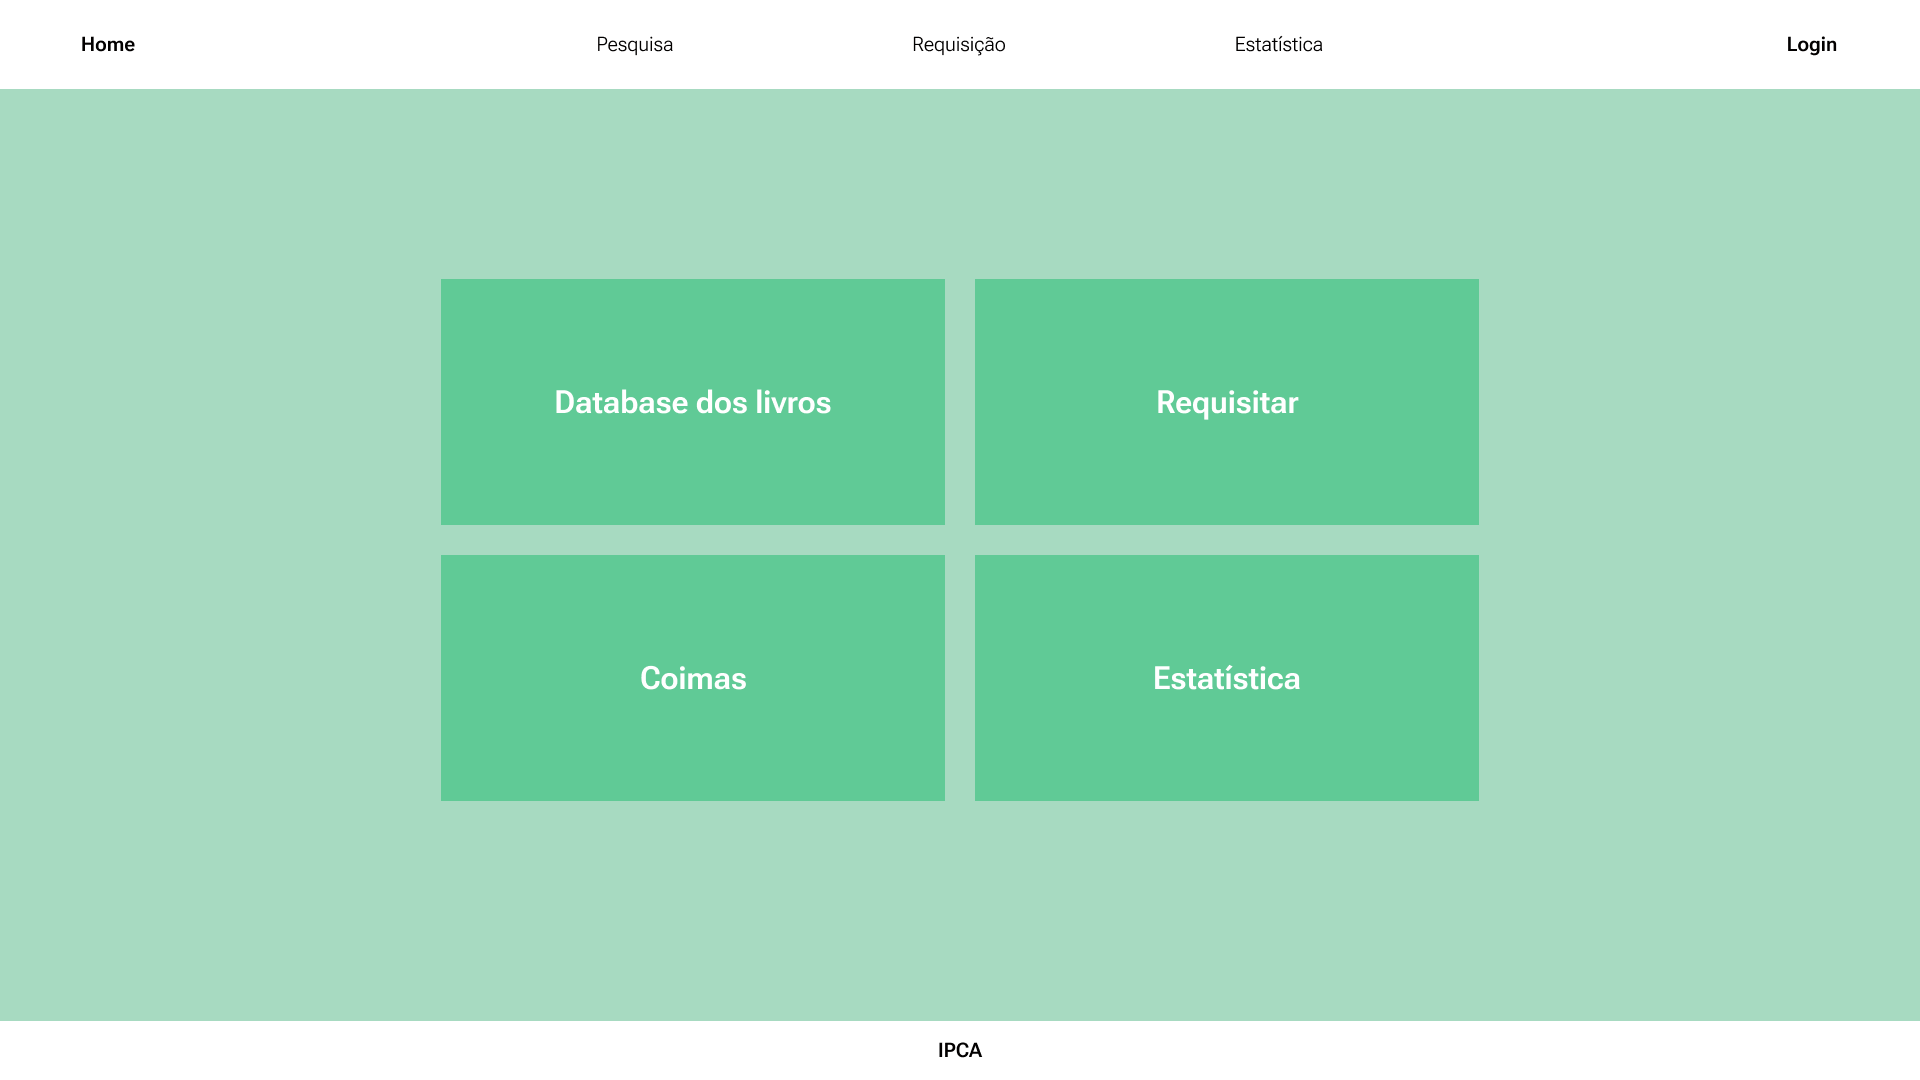
\includegraphics[width=1\linewidth]{../Mockups/PNGs/Home.png}  % largura percentual 
	\caption{\ref{mo:270}}
	\label{fig:chap270}
\end{figure}


\newpage 

\subsection{\labeltext[Ecrã - Sign Up]{Ecrã - Sign Up}{mo:271}}

Nesta página será onde o utilizador faz o seu registo/login. O aluno/funcionario/admin introduzem os seus dados de acesso, e no caso de se esquecerem da password, clicam no texto correspondente.

\begin{figure}[H]
	\centering
	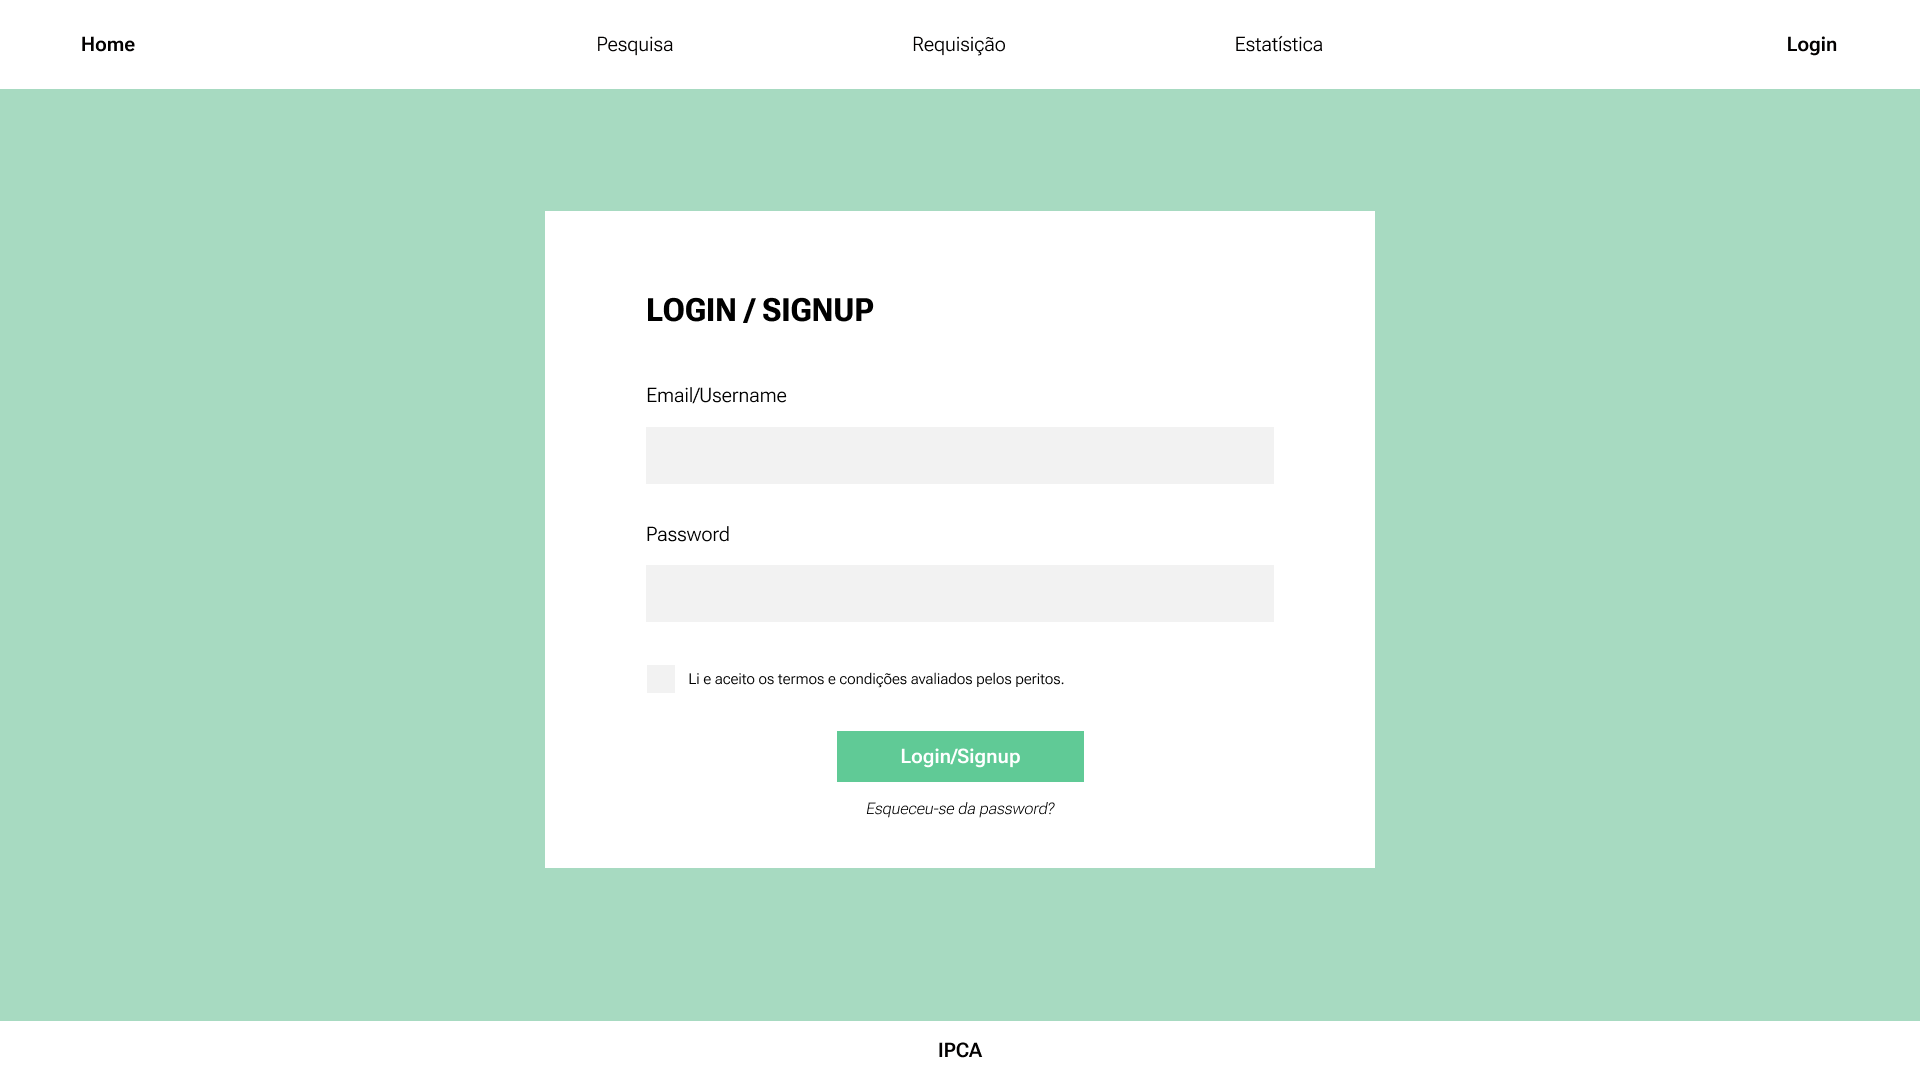
\includegraphics[width=1\linewidth]{../Mockups/PNGs/Login - Signup.png}  % largura percentual 
	\caption{\ref{mo:271}}
	\label{fig:chap271}
\end{figure}


\newpage 

\subsection{\labeltext[Ecrã - Login]{Ecrã - Login}{mo:272}}

Página onde os alunos/funcionarios/admin se encontram, se esquecerem da sua password. Necessita sempre do email por termos de segurança.

\begin{figure}[H]
	\centering
	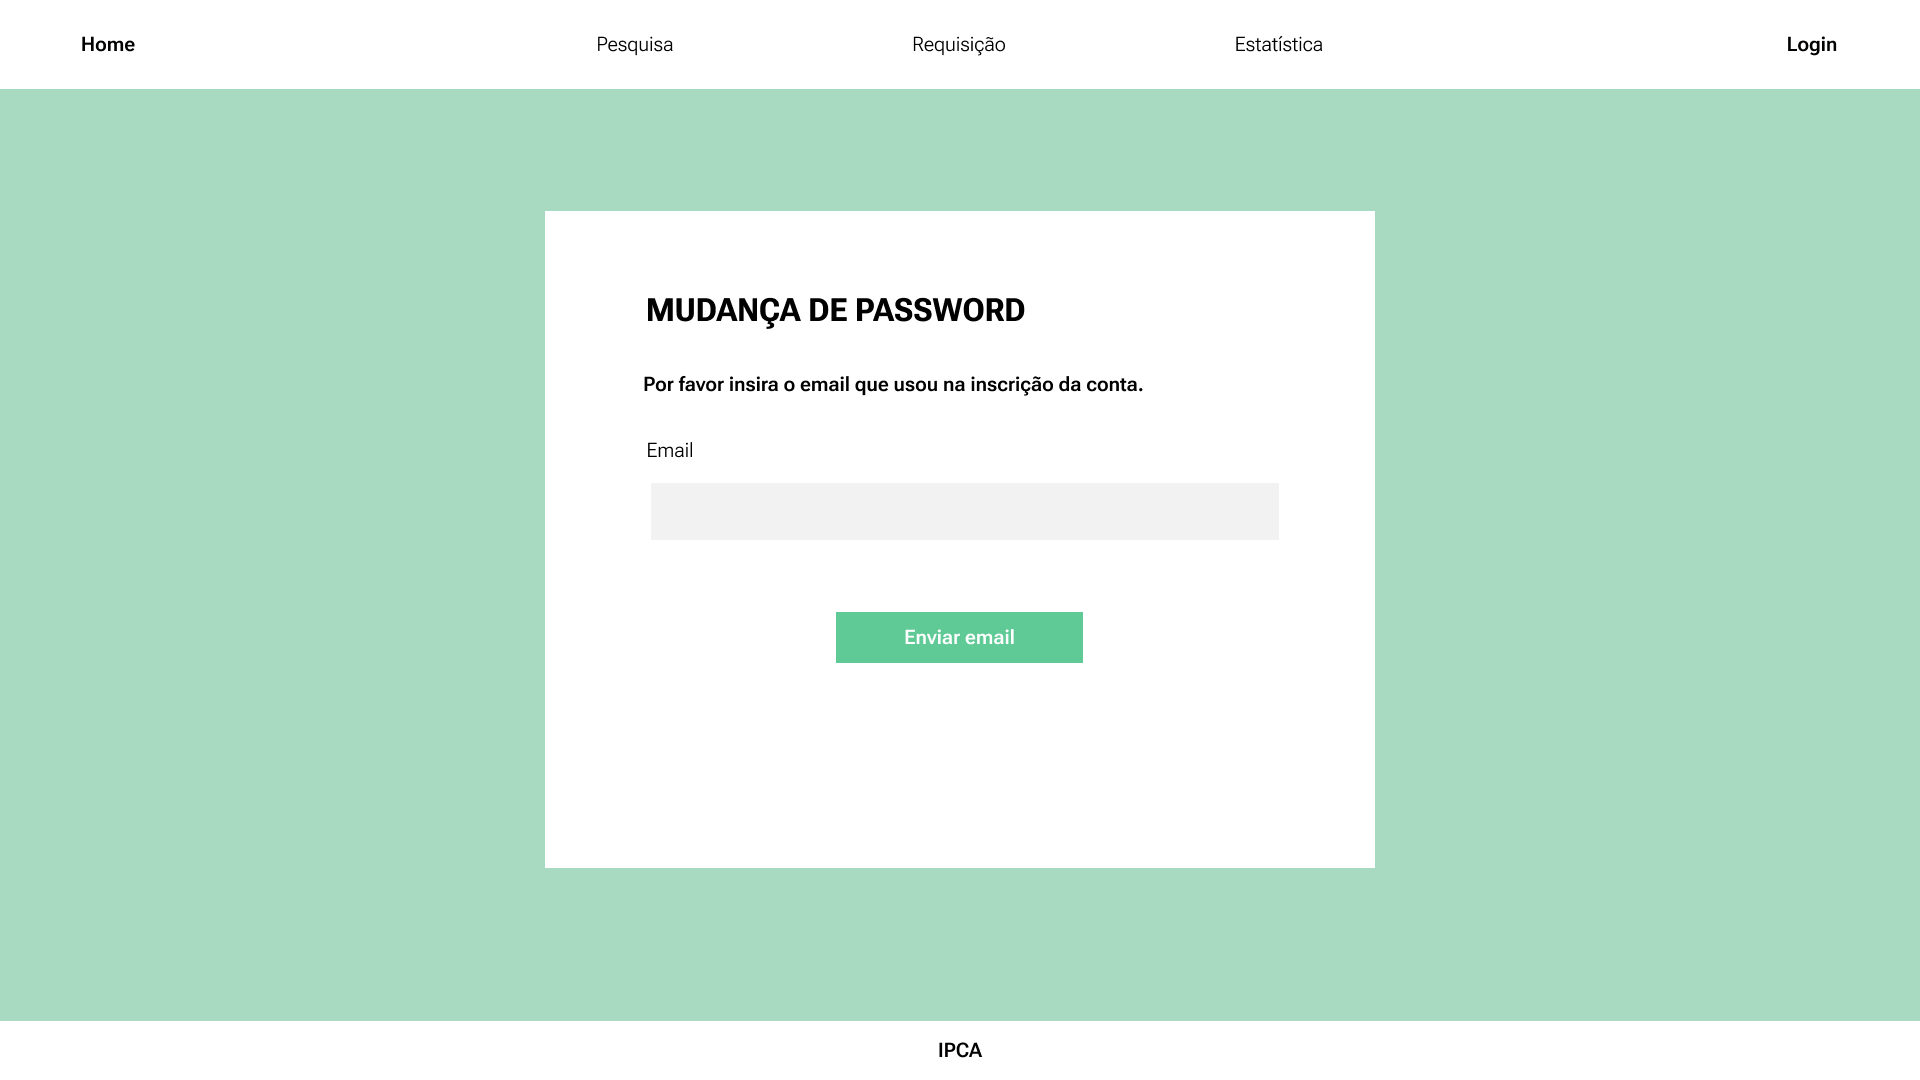
\includegraphics[width=1\linewidth]{../Mockups/PNGs/Login - Password.png}  % largura percentual 
	\caption{\ref{mo:272}}
	\label{fig:chap272}
\end{figure}


\newpage

\subsection{\labeltext[Ecrã - Login Confirmação]{Ecrã - Login Confirmação}{mo:273}}

Pop-up na pagina de Login - Password, a confirmar que o email, foi enviado com smoesso acompanhado de um pequeno aviso caso algo se encontre errado no email.

\begin{figure}[H]
	\centering
	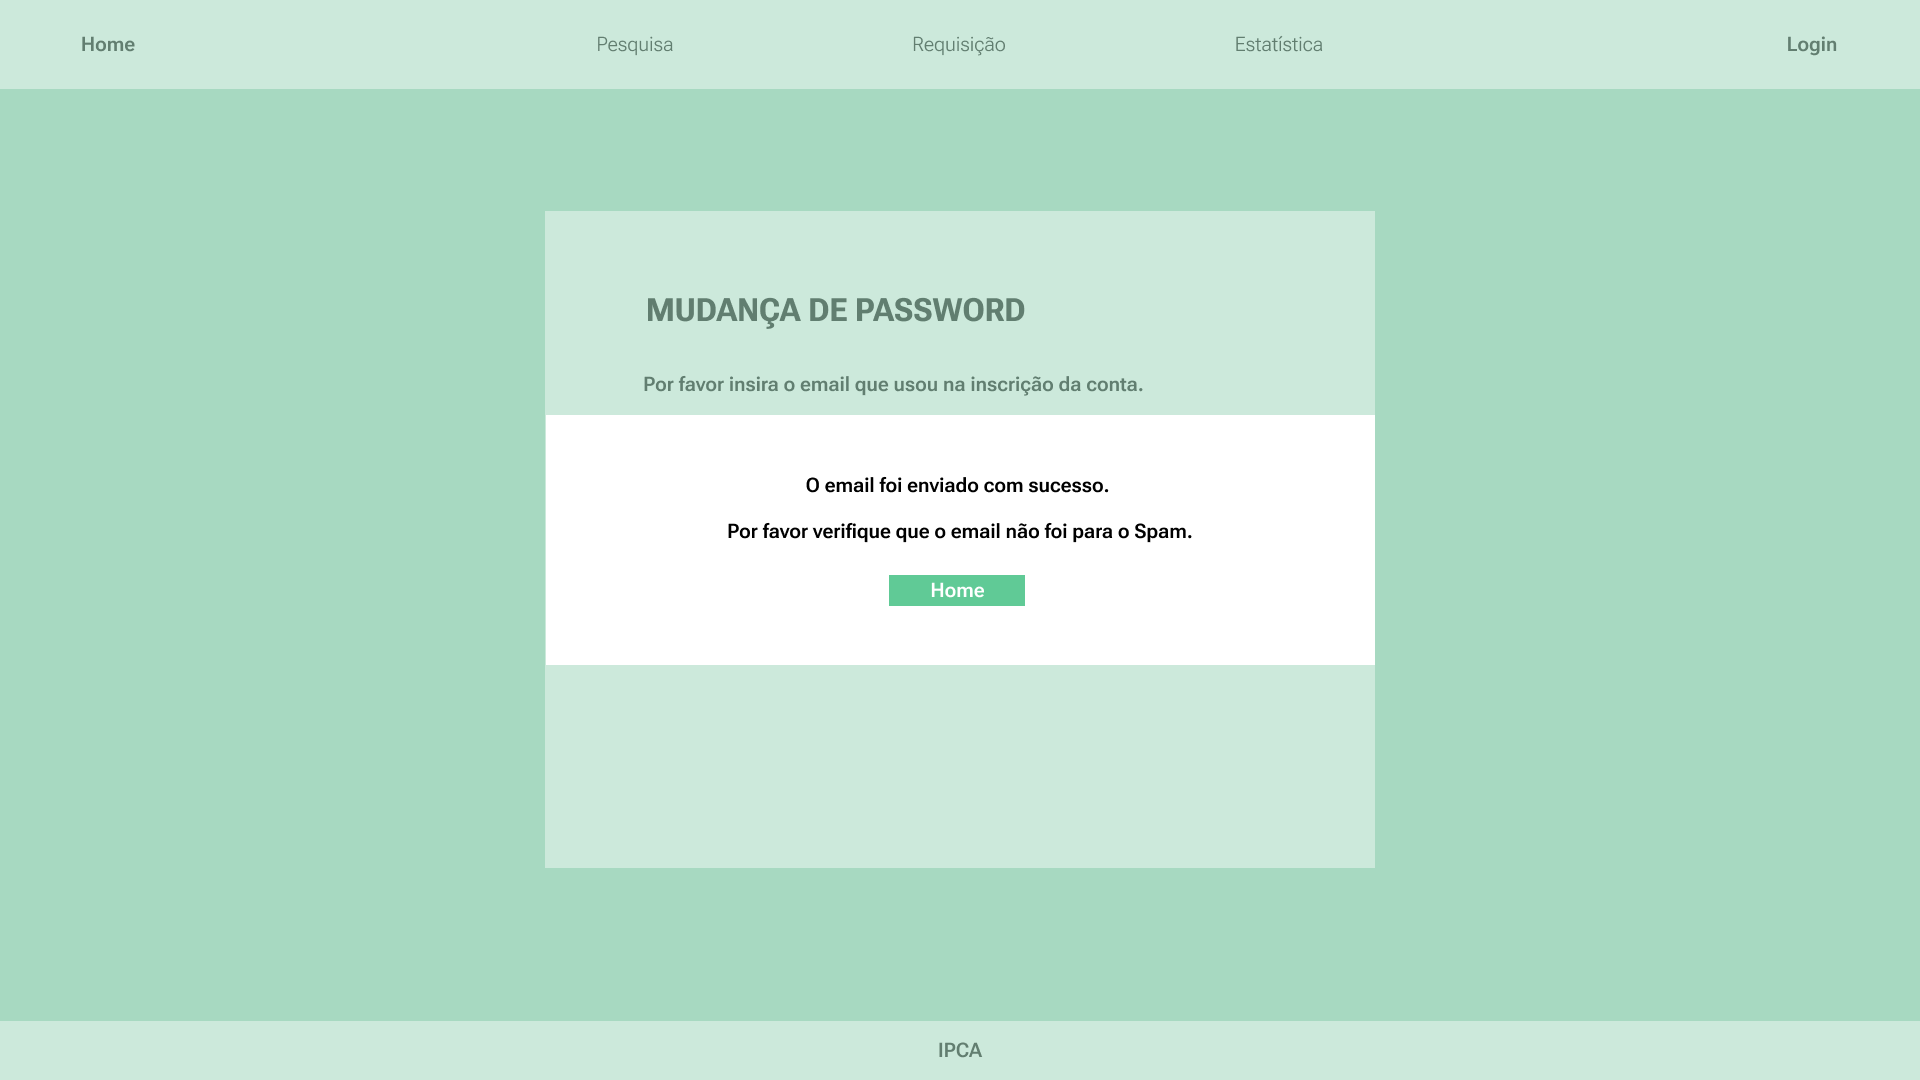
\includegraphics[width=1\linewidth]{../Mockups/PNGs/Login - Password confirmacao.png}  % largura percentual 
	\caption{\ref{mo:273}}
	\label{fig:chap273}
\end{figure}


\newpage 

\subsection{\labeltext[Ecrã - Perfil Utilzador]{Ecrã - Perfil Utilzador}{mo:274}}

A pagina onde o utilizador pode ver a sua informação privada. É possivel também alterar qualquer informação desta pagina caso o mesmo pretenda.

\begin{figure}[H]
	\centering
	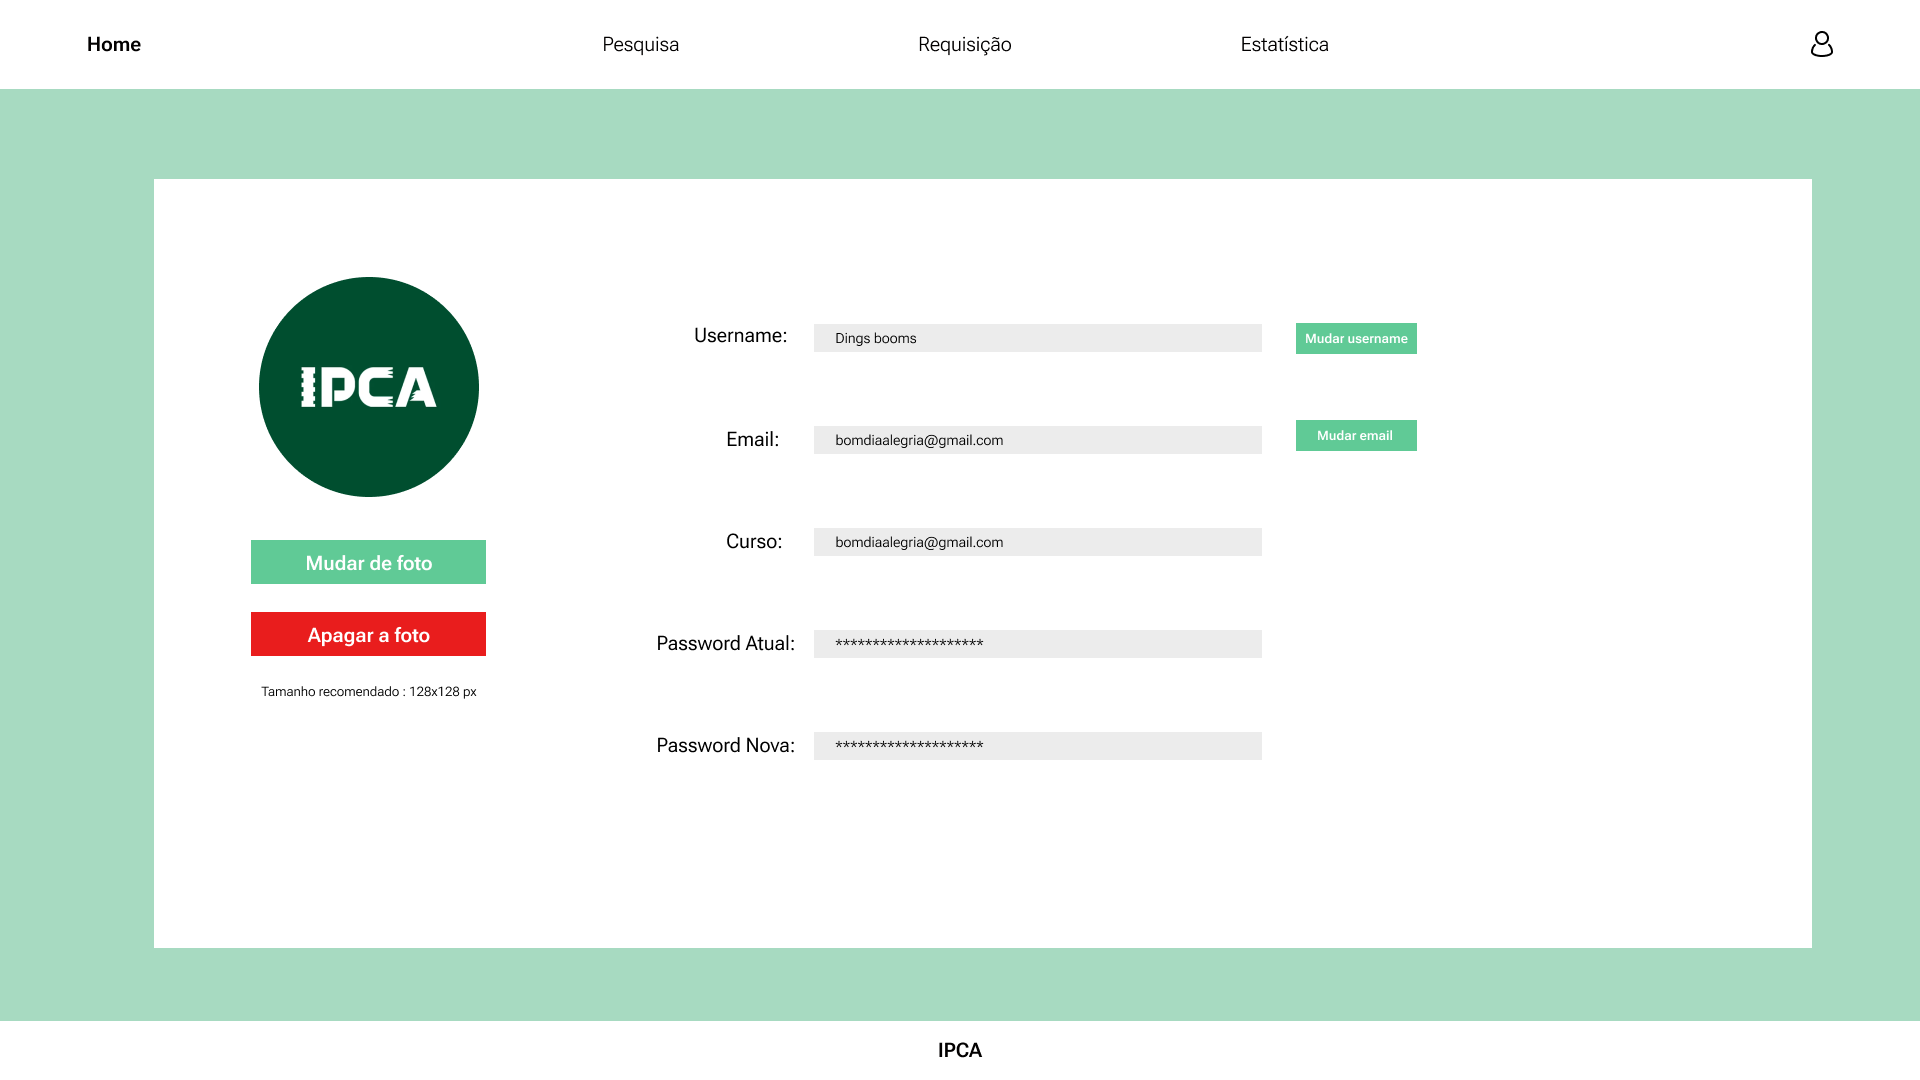
\includegraphics[width=1\linewidth]{../Mockups/PNGs/Perfil do utilizador.png}  % largura percentual 
	\caption{\ref{mo:274}}
	\label{fig:chap274}
\end{figure}

\newpage

\subsection{\labeltext[Ecrã - Pesquisa]{Ecrã - Pesquisa}{mo:275}}

Aqui se encontra a pagina onde é possível fazer a pesquisa dos livros da database e ao mesmo tempo ver se estão disponíveis para serem requisitados. Cada livro vêm com as suas especificações ao lado para o utilizador ver e perceber, se é mesmo o livro que pretendia. 

\begin{figure}[H]
	\centering
	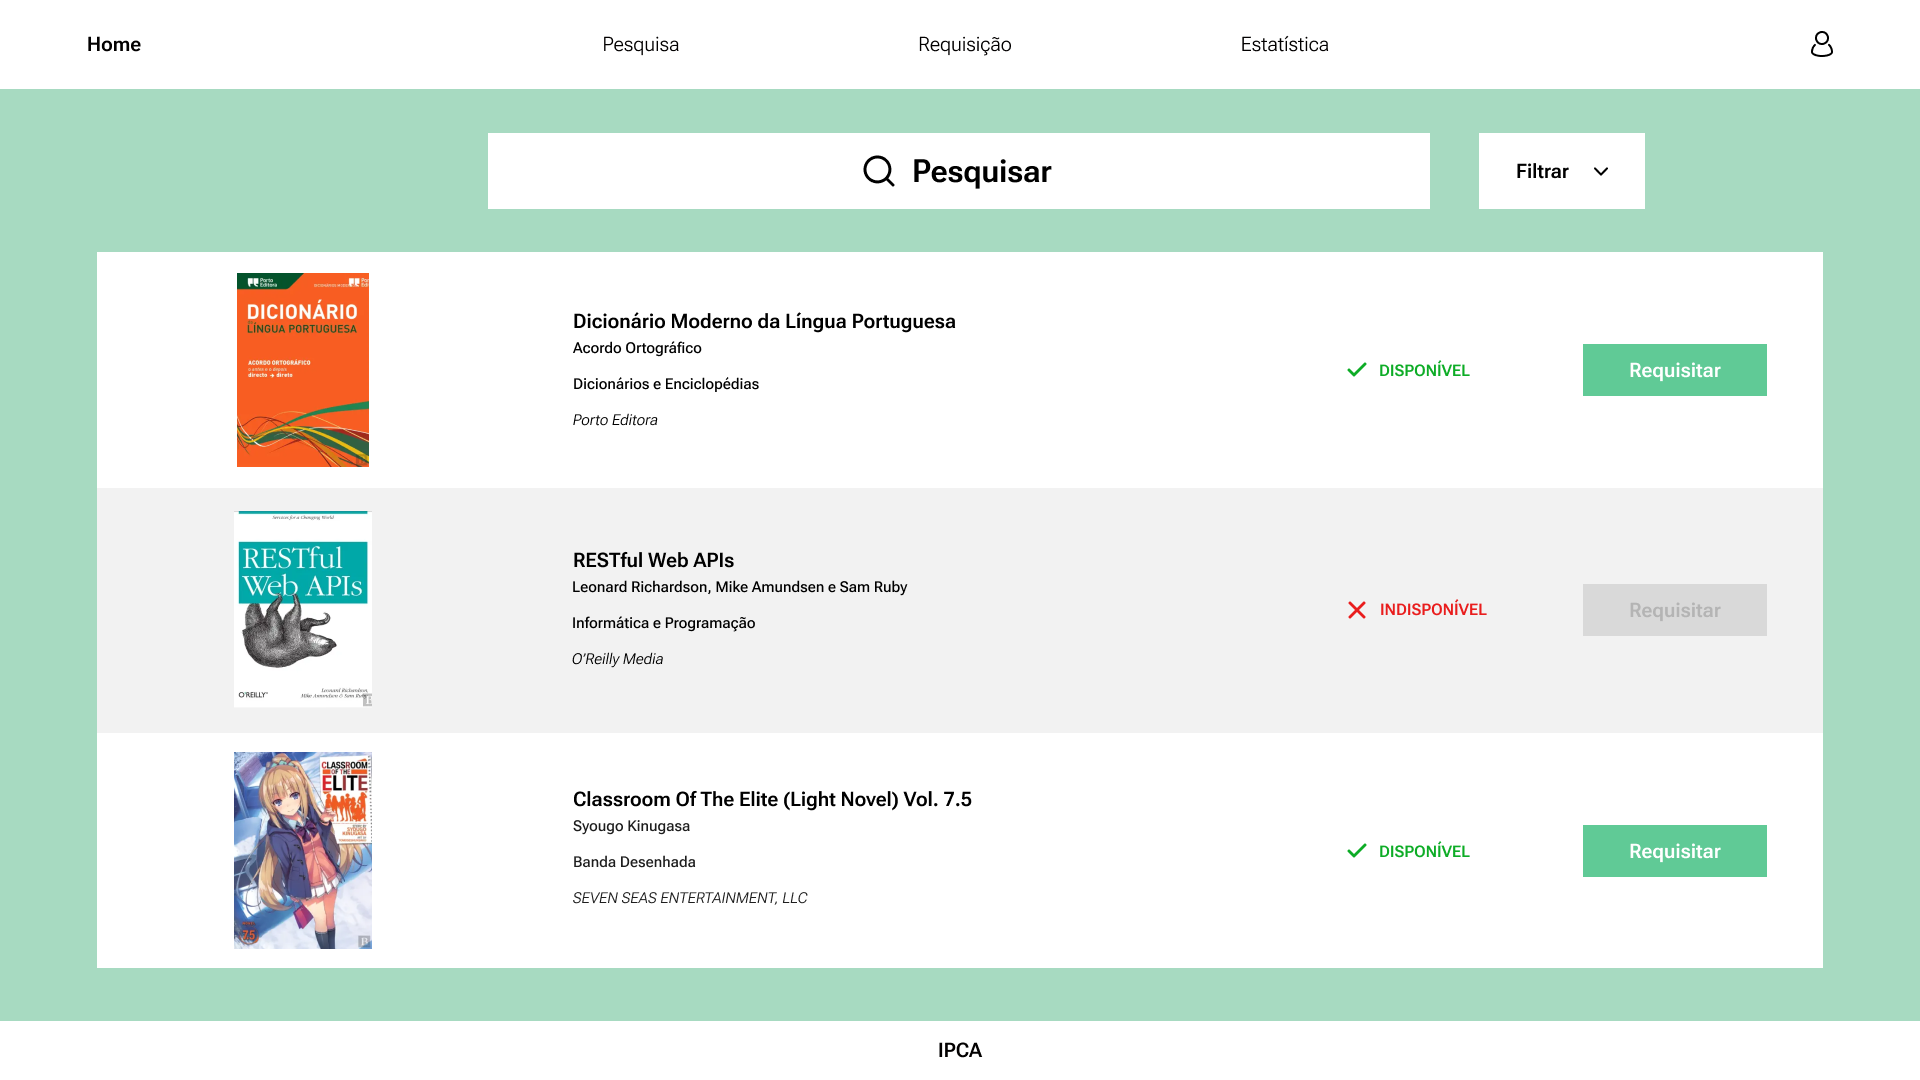
\includegraphics[width=1\linewidth]{../Mockups/PNGs/Pesquisa dos livros.png}  % largura percentual 
	\caption{\ref{mo:275}}
	\label{fig:chap275}
\end{figure}

\newpage 

\subsection{\labeltext[Ecrã - Requisição]{Ecrã - Requisição}{mo:276}}

Pop-up da página anterior onde é escolhido a data de entrega e de limite da requisição como também o numero de exemplares que pretende requisitar.

\begin{figure}[H]
	\centering
	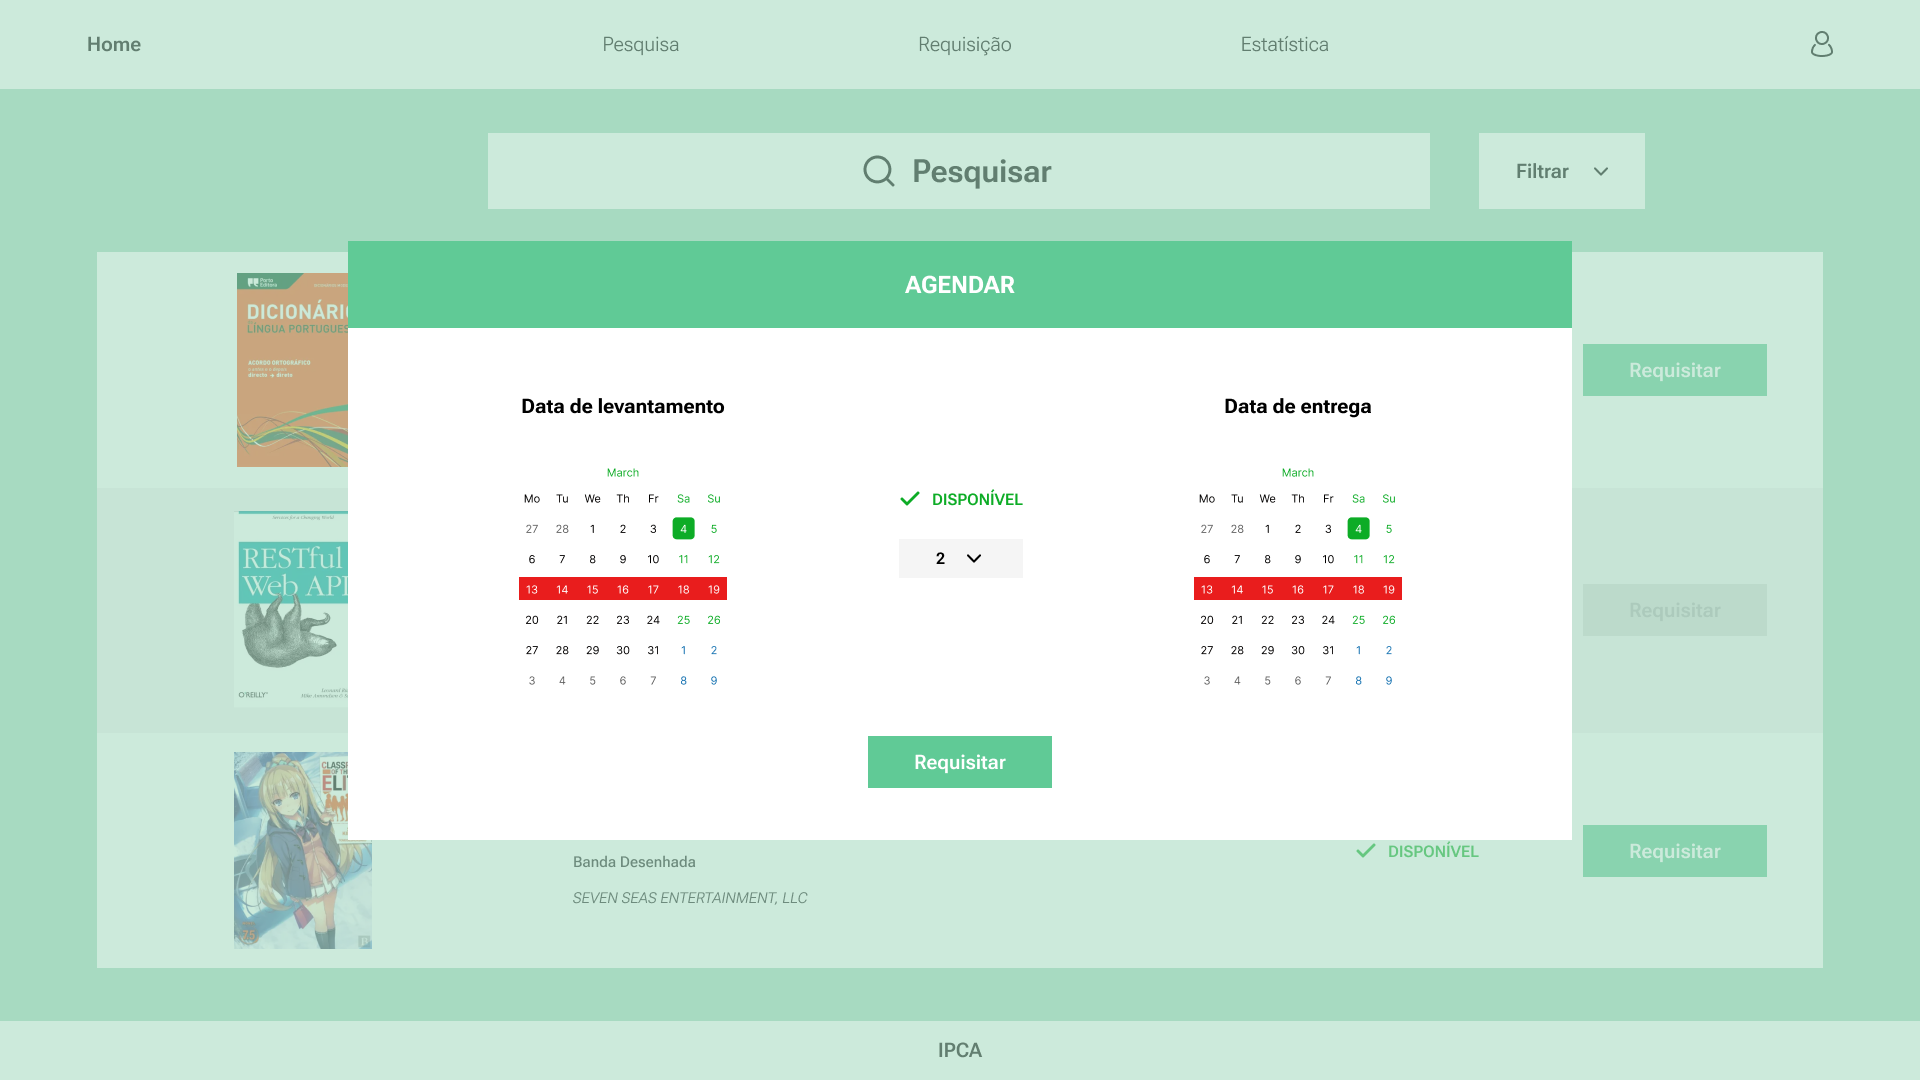
\includegraphics[width=1\linewidth]{../Mockups/PNGs/Agendar Requisitar.png}  % largura percentual 
	\caption{\ref{mo:276}}
	\label{fig:chap276}
\end{figure}


\newpage

\subsection{\labeltext[Ecrã - Minhas Requisições]{Ecrã - Requisições}{mo:277}}

Pagina do utilizador, onde encontram-se as requisições feitas pelo mesmo. Coimas e data de limite da requisição aparecem nesta pagina e as coimas são pagas nesta página ao cliquar no "Expirou".

\begin{figure}[H]
	\centering
	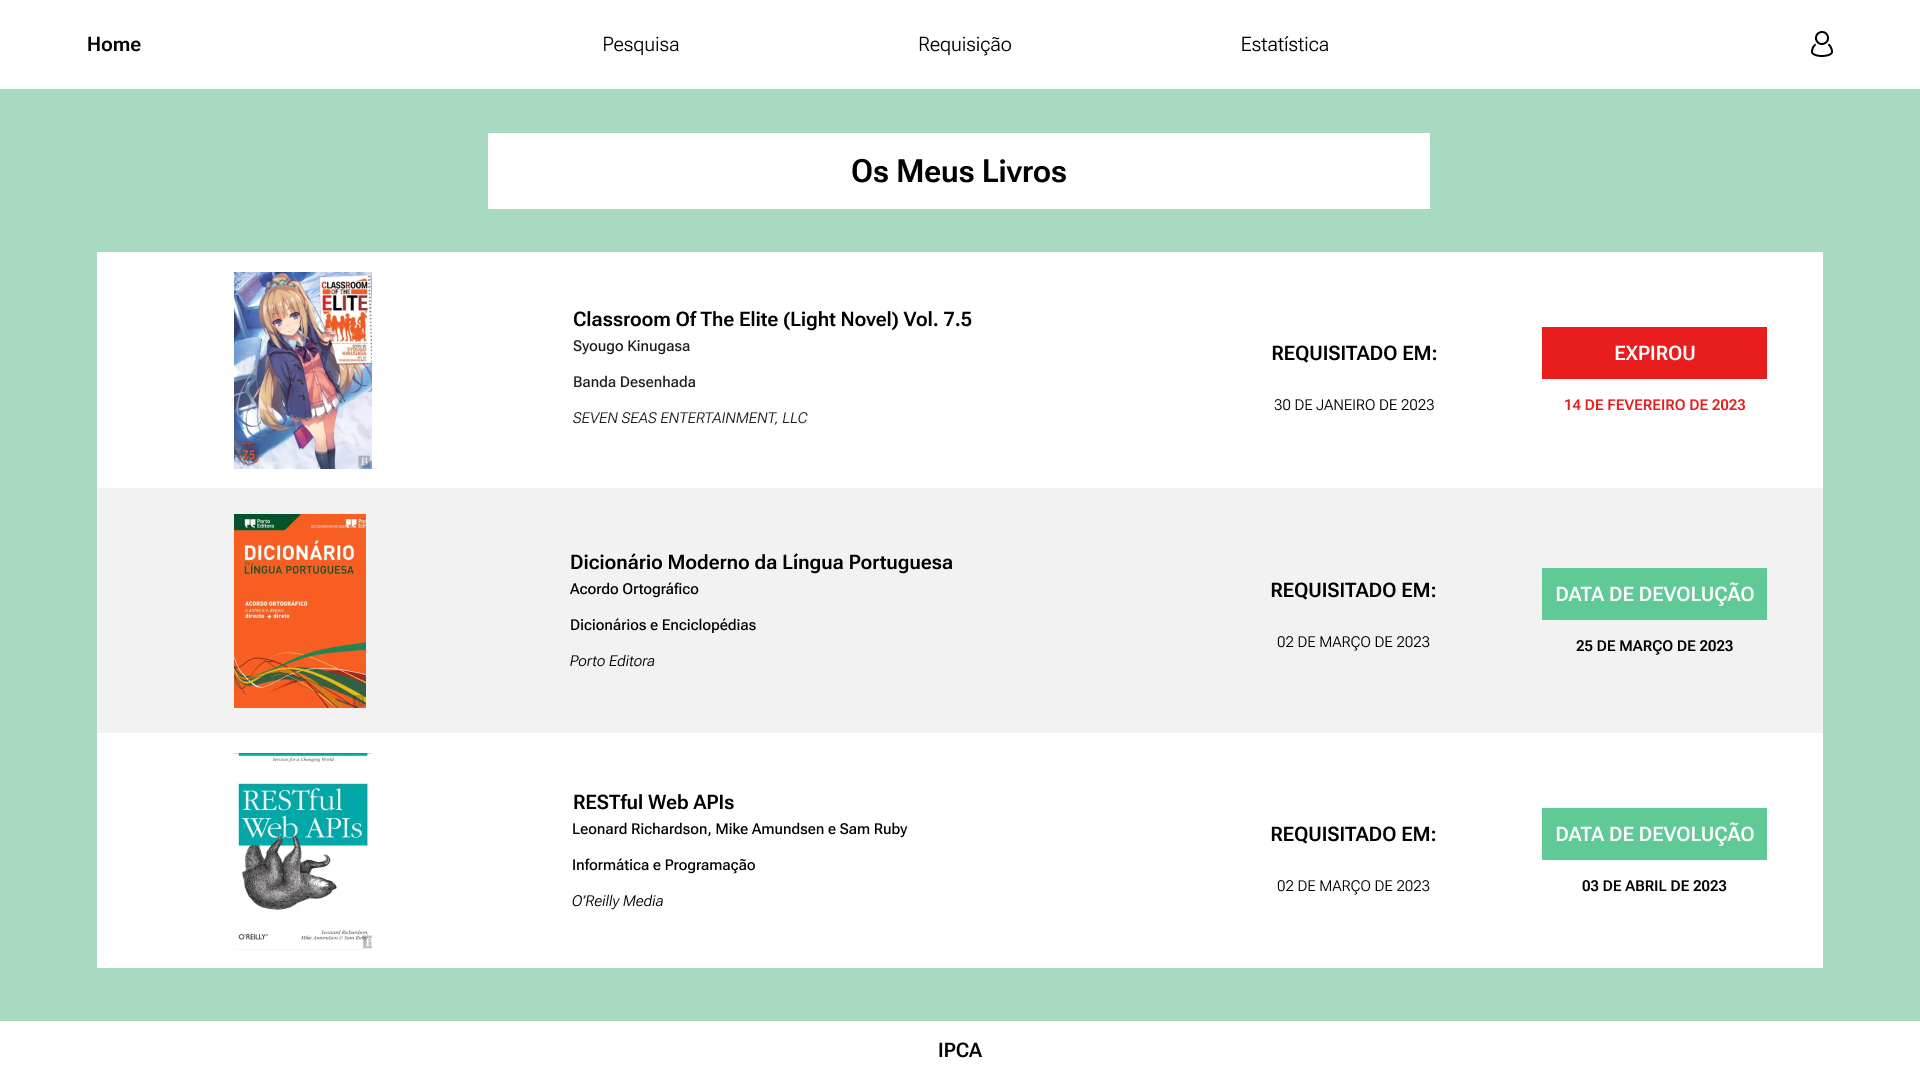
\includegraphics[width=1\linewidth]{../Mockups/PNGs/Minhas Requisicoes.png}  % largura percentual 
	\caption{\ref{mo:277}}
	\label{fig:chap277}
\end{figure}


\newpage

\subsection{\labeltext[Ecrã - Pagamento Multibanco]{Ecrã - Pagamento Multibanco}{mo:278}}

Pop-up da página das "Minhas Requisições" onde vão ser pagas as coimas. Neste ponto é especificado o pagamento por Multibanco.

\begin{figure}[H]
	\centering
	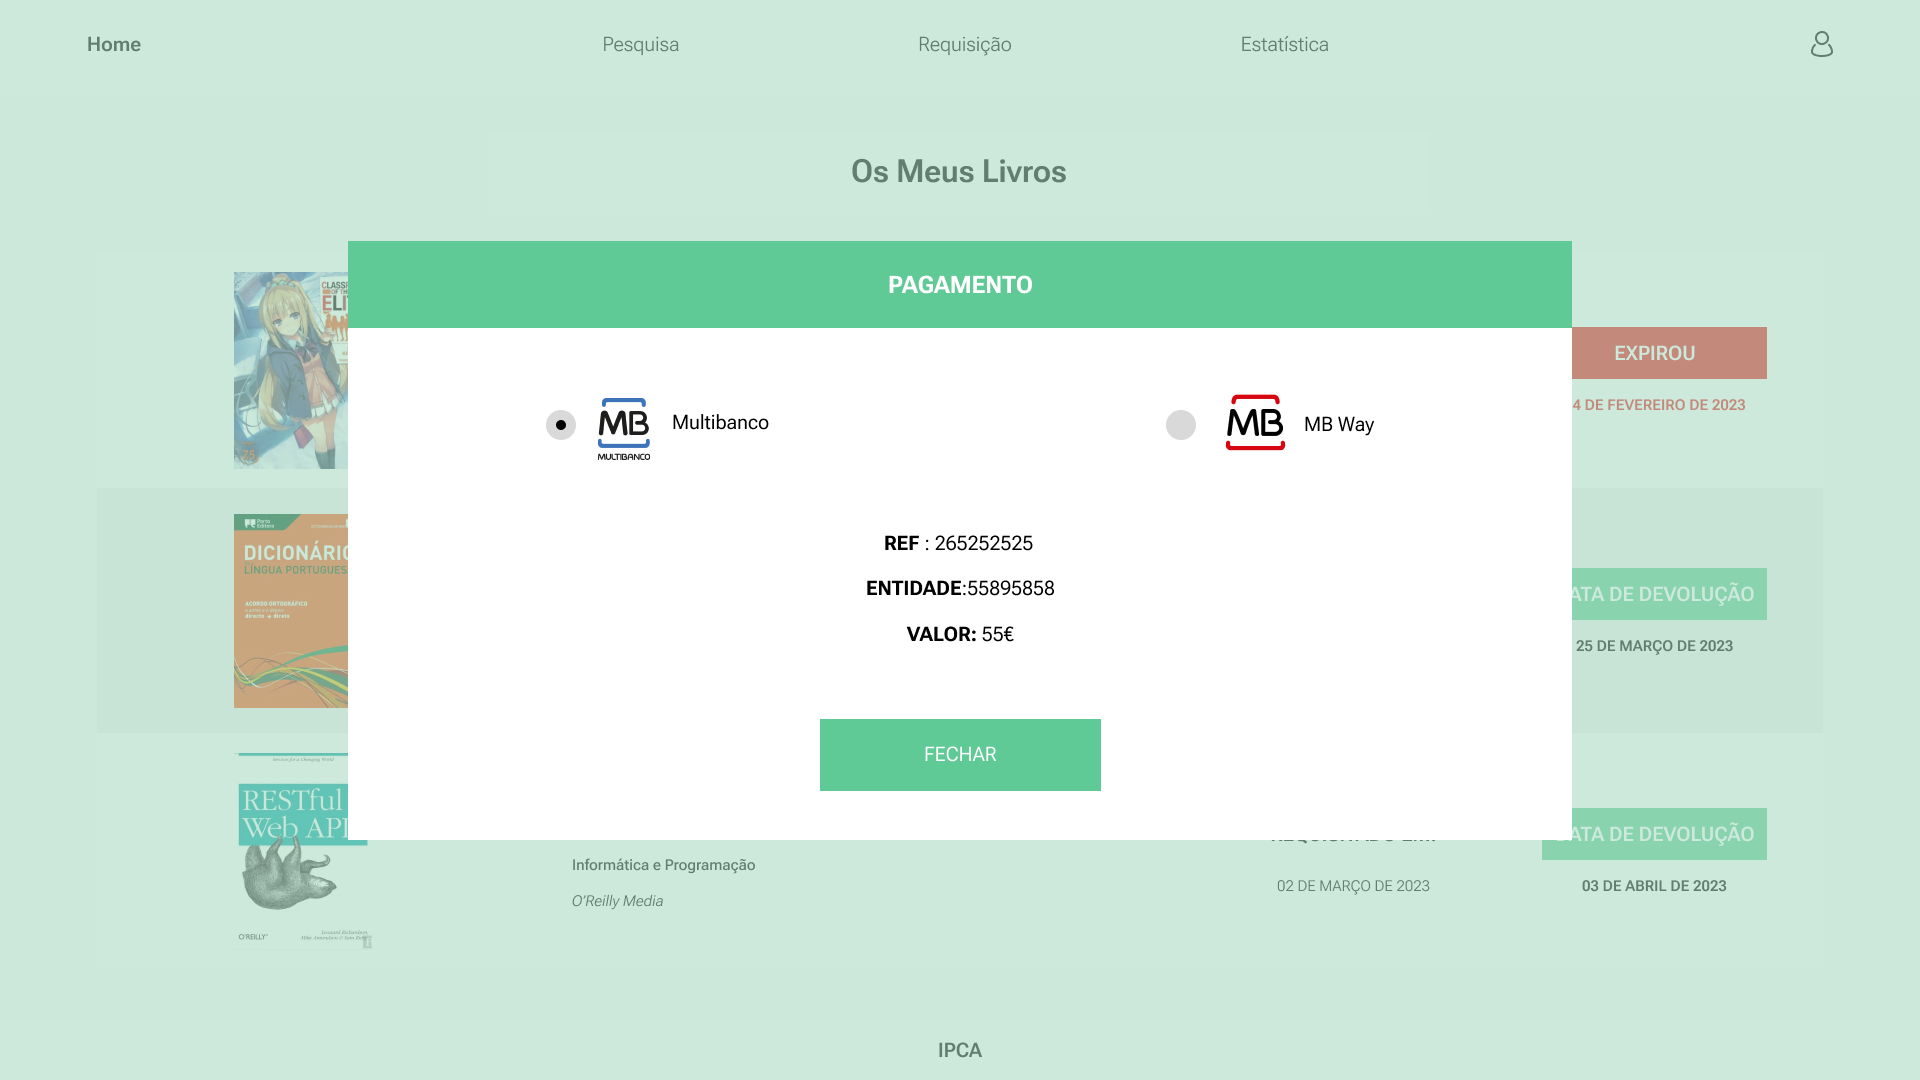
\includegraphics[width=1\linewidth]{../Mockups/PNGs/Pagamento de coimas Multibanco.png}  % largura percentual 
	\caption{\ref{mo:278}}
	\label{fig:chap278}
\end{figure}


\newpage

\subsection{\labeltext[Ecrã - Pagamento MBWay]{Ecrã - Pagamento MBWay}{mo:279}}

Pop-up da página das "Minhas Requisições" onde vão ser pagas as coimas. Neste ponto é especificado o pagamento por MBWay.

\begin{figure}[H]
	\centering
	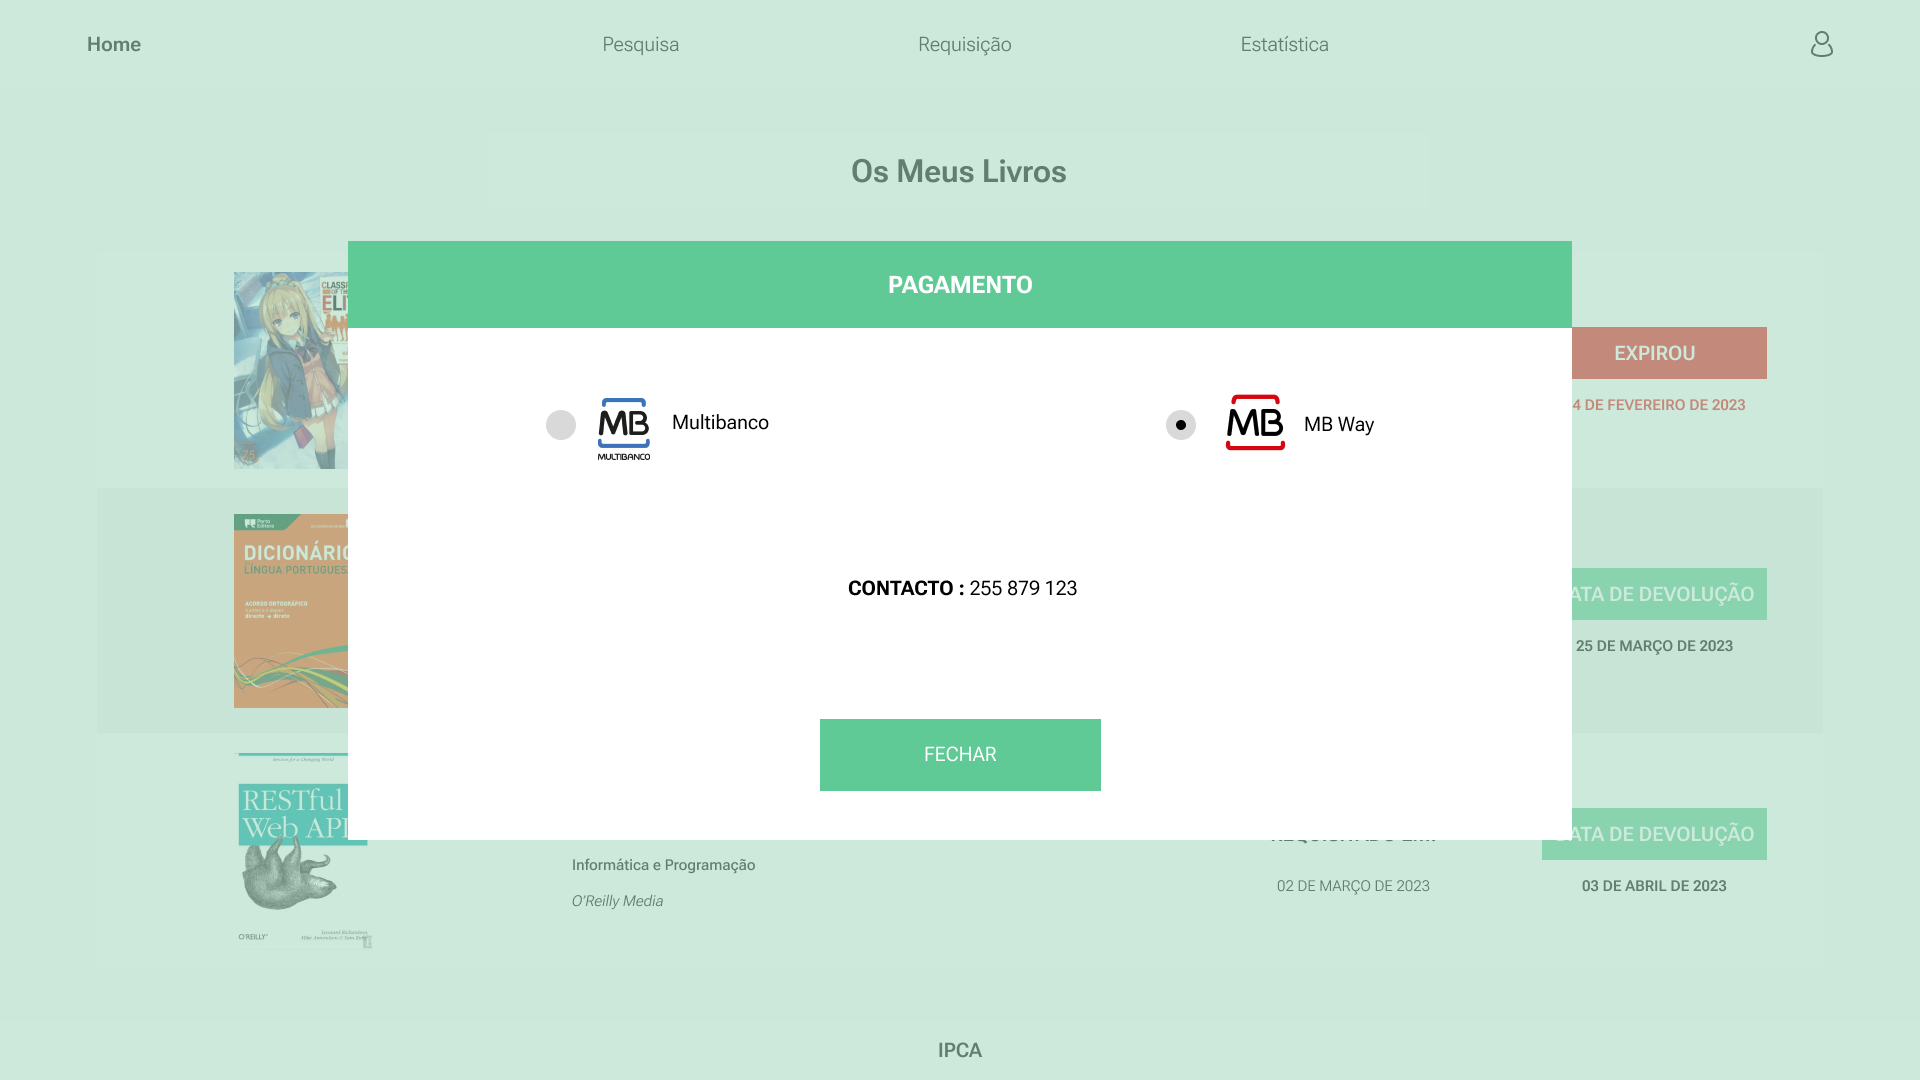
\includegraphics[width=1\linewidth]{../Mockups/PNGs/Pagamento de coimas MBWay.png}  % largura percentual 
	\caption{\ref{mo:279}}
	\label{fig:chap279}
\end{figure}


\newpage

\subsection{\labeltext[Ecrã - Análise de dados 1]{Ecrã - Análise de dados 1}{mo:280}}

Pagina web onde entra a análise e estudo sobre a biblioteca, neste caso em específico uma representação de um gráfico de barras, com uma pequena lista ao seu lado.

\begin{figure}[H]
	\centering
	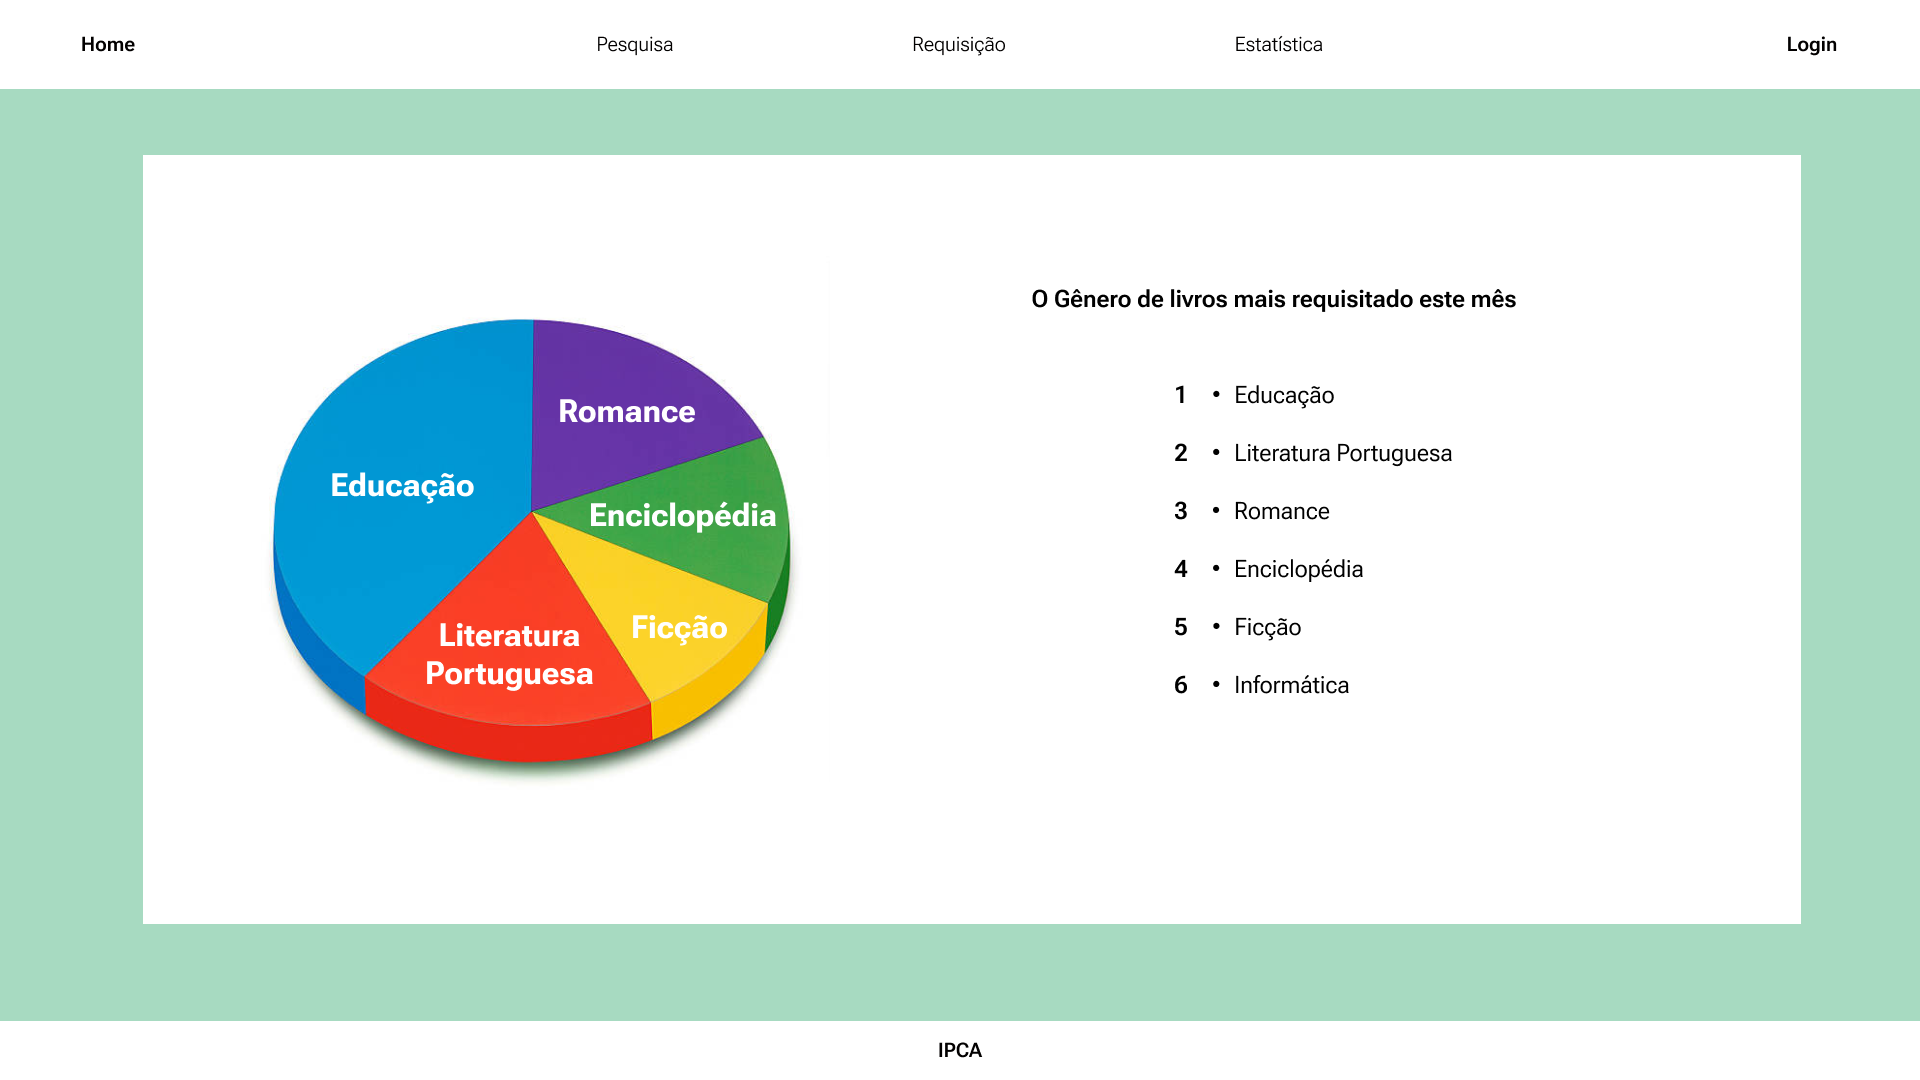
\includegraphics[width=1\linewidth]{../Mockups/PNGs/Estatistica circulo.png}  % largura percentual 
	\caption{\ref{mo:280}}
	\label{fig:chap280}
\end{figure}



\newpage

\subsection{\labeltext[Ecrã - Análise de dados 2]{Ecrã - Análise de dados 2}{mo:281}}

Pagina web onde entra a análise e estudo sobre a biblioteca, neste caso em específico uma representação de um gráfico de barras sobre o estudo do passado ano na biblioteca.

\begin{figure}[H]
	\centering
	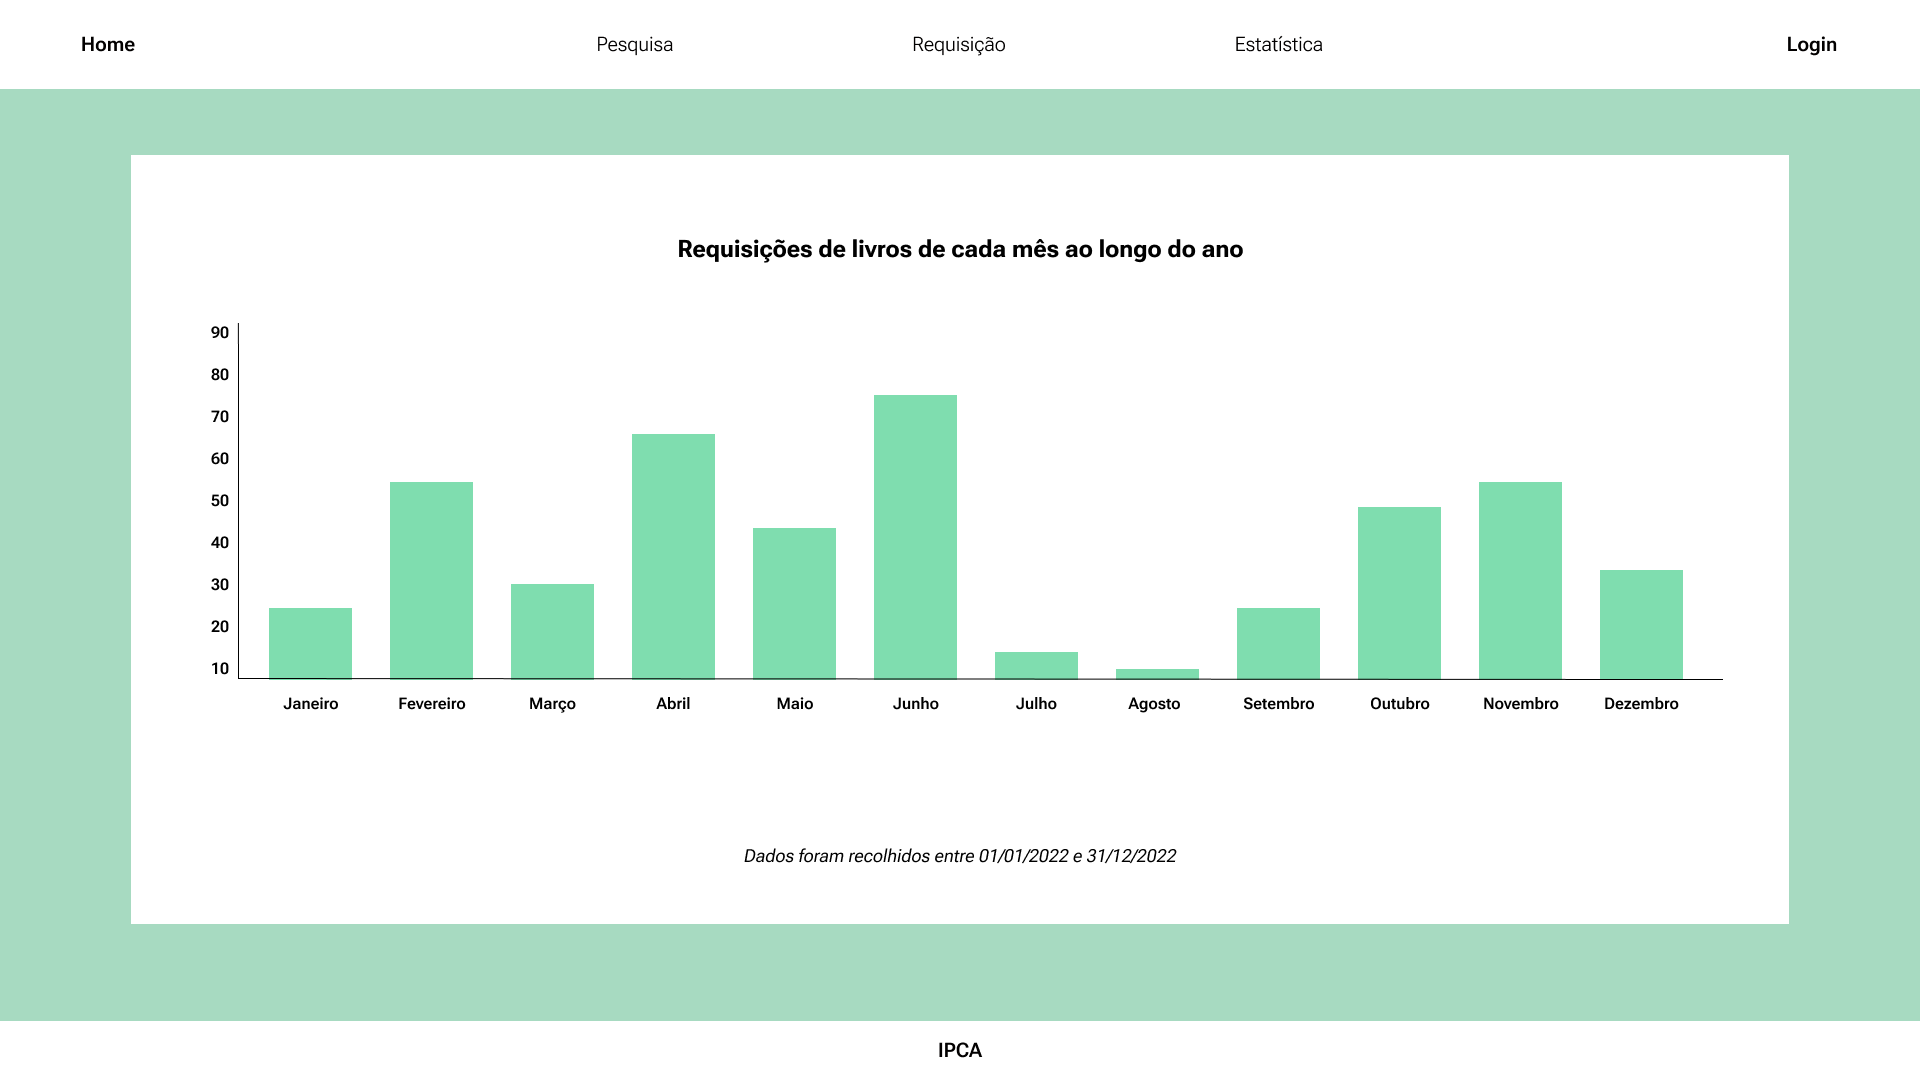
\includegraphics[width=1\linewidth]{../Mockups/PNGs/Estatistica barras.png}  % largura percentual 
	\caption{\ref{mo:281}}
	\label{fig:chap281}
\end{figure}
